%%%%%%%%%%%%%%%%%%%%%%%%%%%%%%%%%%%%%%%%%
%
% (c) 2019 by Jennifer Laaser
%
% This work is licensed under the Creative Commons Attribution-NonCommercial-ShareAlike 4.0 International License. To view a copy of this license, visit http://creativecommons.org/licenses/by-nc-sa/4.0/ or send a letter to Creative Commons, PO Box 1866, Mountain View, CA 94042, USA.
%
% The current source for these materials is accessible on Github: https://github.com/jlaaser/pogil-polymers
%
%%%%%%%%%%%%%%%%%%%%%%%%%%%%%%%%%%%%%%%%%

\documentclass[instructor,handout]{pogil}

%%%%%%%%%%%%%%%%% DOCUMENT INFORMATION %%%%%%%%%%%%%%%%%%%%%%%%

\copyrightshort{
\includegraphics[width=0.1\textwidth]{by-nc-sa} J. Laaser 2019}

%%%%%%%%%%%%%%%%%%%%%%%%%%%%%%%%%%%%%%%%%%%%%%%%%%%%%%%%%%%%%%%%%
%%%%%%%%%%%%%%%%%%%%%%%%%%%%%%%%%%%%%%%%%%%%%%%%%%%%%%%%%%%%%%%%%

\begin{document}
	
% to change the activity output in the pdf, change this to the file path for the activity you want to include:
%%%%%%%%%%%%%%%%%%%%%%%%%%%%%%%%%%%%%%%%%%
%
% (c) 2018 by Jennifer Laaser
%
% This work is licensed under the Creative Commons Attribution-NonCommercial-ShareAlike 4.0 International License. To view a copy of this license, visit http://creativecommons.org/licenses/by-nc-sa/4.0/ or send a letter to Creative Commons, PO Box 1866, Mountain View, CA 94042, USA.
%
% The current source for these materials is accessible on Github: https://github.com/jlaaser/pogil-polymers
%
%%%%%%%%%%%%%%%%%%%%%%%%%%%%%%%%%%%%%%%%%

\section{Activity Template}
\renewcommand{\figpath}{content/figs}

\textbf{Focus question:} Put a central question for the students to consider through this exercise here.

\subsection{Model 1:  ABC}

Here is the first model for students to consider

% to include images, put them in the folder specified by figpath and then use:
%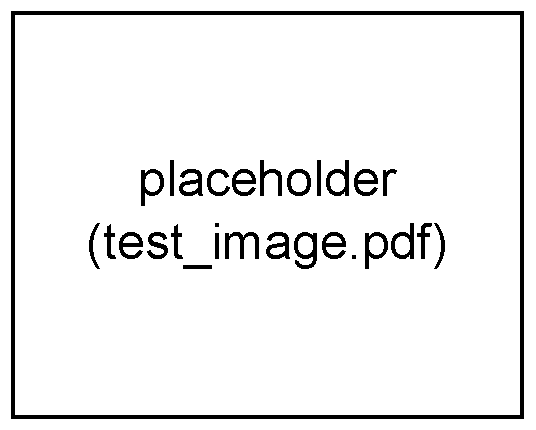
\includegraphics[width=0.8\textwidth]{\figpath/test_image.pdf}

\subsection{Critical Thinking Questions}

	\begin{enumerate}
		\item First question?
		\item Second question?
	\end{enumerate}

\subsection{Model 2: DEF}

\subsection{Critical Thinking Questions}

	\begin{enumerate}
		\item First question?
		\item Second question?
	\end{enumerate}

\subsection{Exercises}

	After class, \textbf{read} the following sections of your textbook:
	
	\begin{enumerate}
		\item First section
		\item Second section
	\end{enumerate}
	
	Then, do the following exercises:
	
	\begin{enumerate}
		\item First exercise
		\item Second exercise
	\end{enumerate}
%%%%%%%%%%%%%%%%%%%%%%%%%%%%%%%%%%%%%%%%%
%
% (c) 2018 by Jennifer Laaser
%
% This work is licensed under the Creative Commons Attribution-NonCommercial-ShareAlike 4.0 International License. To view a copy of this license, visit http://creativecommons.org/licenses/by-nc-sa/4.0/ or send a letter to Creative Commons, PO Box 1866, Mountain View, CA 94042, USA.
%
% The current source for these materials is accessible on Github: https://github.com/jlaaser/pogil-polymers
%
%%%%%%%%%%%%%%%%%%%%%%%%%%%%%%%%%%%%%%%%%

\renewcommand{\figpath}{content/polymphys/solution-thermo/phase-diagrams/figs}

\begin{activity}[Phase Diagrams of Polymer Solutions]

\begin{instructornotes}

	This activity introduces students to key concepts related to phase diagrams of polymer solutions.
	
	After completing this activity, students will be able to:
			\begin{enumerate}
				\item ...
			\end{enumerate}
	This activity will prepare students for ...
			
	\subsection*{Activity summary:}
	\begin{itemize}
		\item \textbf{Activity type:} Learning Cycle
		\item \textbf{Content goals:} Phase diagrams of polymer solutions
		\item \textbf{Process goals:} %https://pogil.org/uploads/attachments/cj54b5yts006cklx4hh758htf-process-skills-official-pogil-list-2015-original.pdf
			written communication, critical thinking, information processing
		\item \textbf{Duration:} TBD
		\item \textbf{Instructor preparation required:} none beyond knowledge of relevant content
		\item \textbf{Related textbook chapters:}
			\begin{itemize}
				\item \emph{Polymer Chemistry} (Hiemenz \& Lodge): sections XX \& YY
			\end{itemize}
	\end{itemize}

\end{instructornotes}

	%\textbf{Focus question:} Put a central question for the students to consider through this exercise here.

\begin{model}[Free-Energy Curves for Polymer Solutions]

According to Flory-Huggins theory, the free energy of a polymer solution is
\begin{equation*}
	\frac{\Delta G_{mix}^{(int)}}{kT} = \phi_1 \phi_2 \chi + \phi_1 \ln \phi_1 + \frac{\phi_2}{N}\ln \phi_2
\end{equation*}
where $\phi_1$ and $\phi_2$ are the volume fractions of solvent and polymer, respectively, $N$ is the degree of polymerization of the polymer, and $\chi$ is the interaction parameter.

The three terms in this expression, plotted against $\phi_1$ (recall that $\phi_2=1-\phi_1$), have the following individual shapes:

\centerline{
	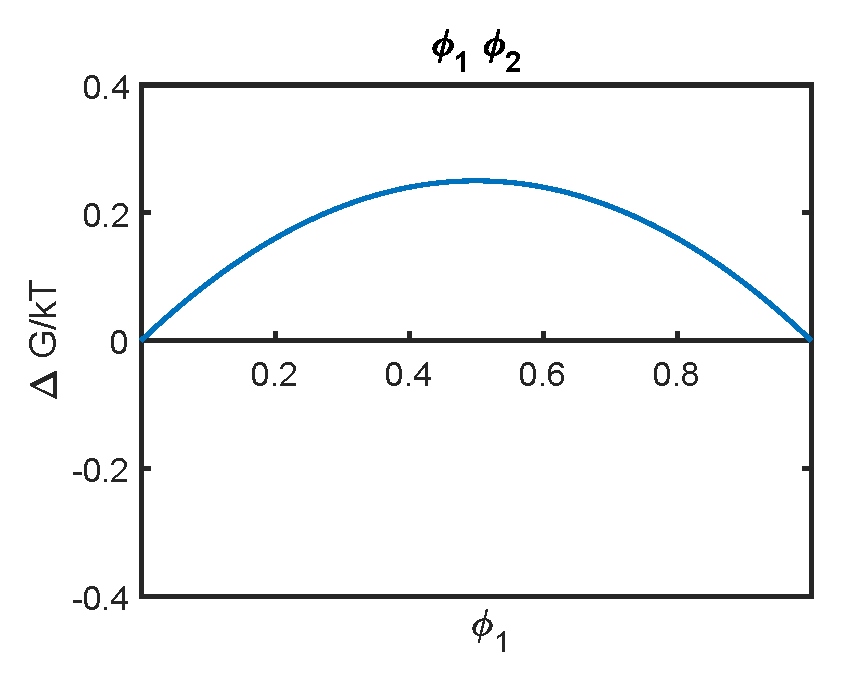
\includegraphics[width=0.4\textwidth]{\figpath/model1-phi1phi2}}
	
\centerline{
	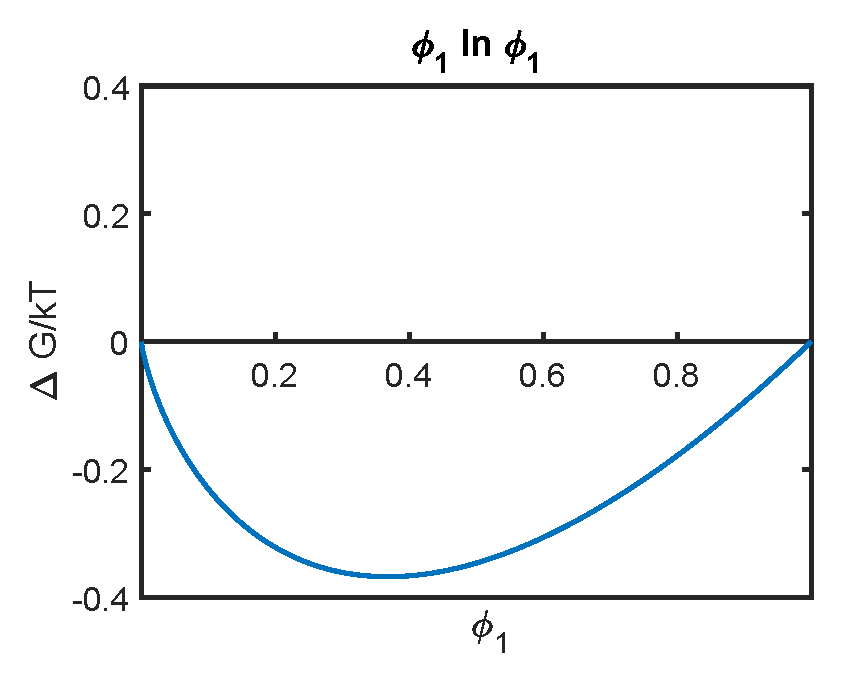
\includegraphics[width=0.4\textwidth]{\figpath/model1-phi1lnphi1}
	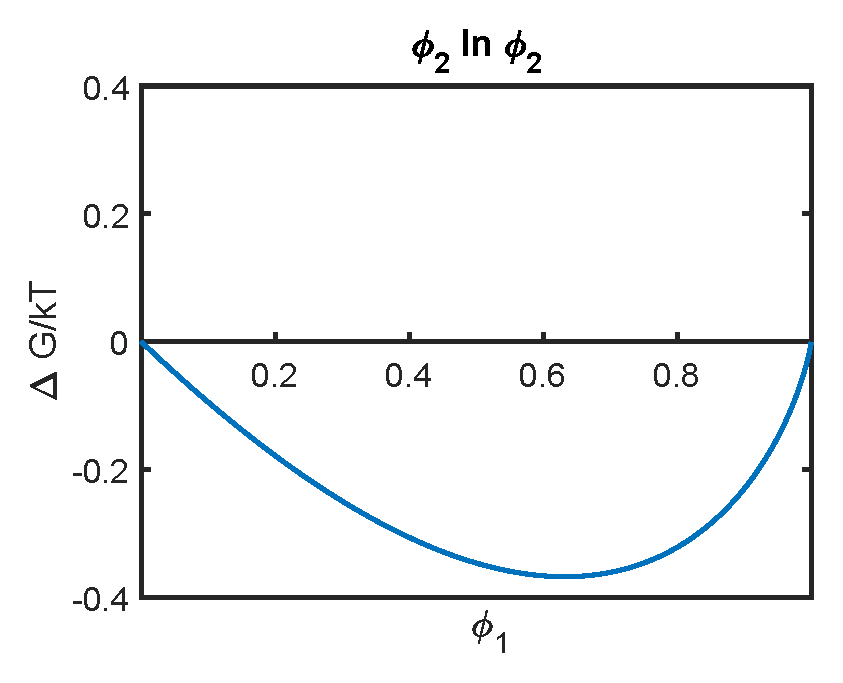
\includegraphics[width=0.4\textwidth]{\figpath/model1-phi2lnphi2}
}

\end{model}

%\vspace{0.05in}
\begin{ctqs}

	\question Sketch the shape of $\frac{\Delta G}{kT}$ that you expect to obtain for each of the following $(\chi,N)$ pairs.  Your plots do not need to be quantitatively accurate, but should capture all of the relevant features.
	
		\vspace{0.05in}
		\begin{minipage}{0.3\textwidth}
			\centerline{$\chi = 0$, $N = 1$}
			
			\centerline{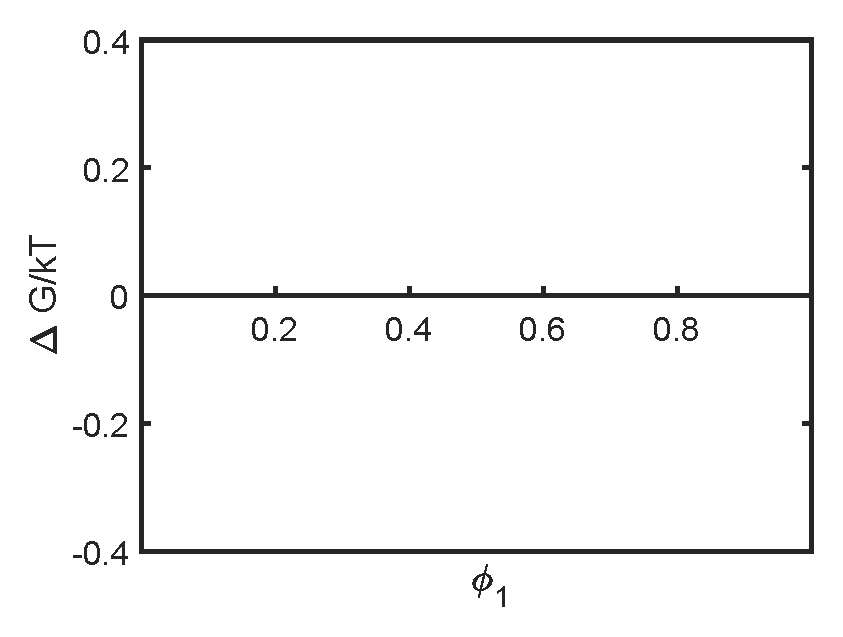
\includegraphics[width=\textwidth]{\figpath/model1-blankaxes}}
		\end{minipage}
		\begin{minipage}{0.3\textwidth}
			\centerline{$\chi = 0$, $N = 2$}
			
			\centerline{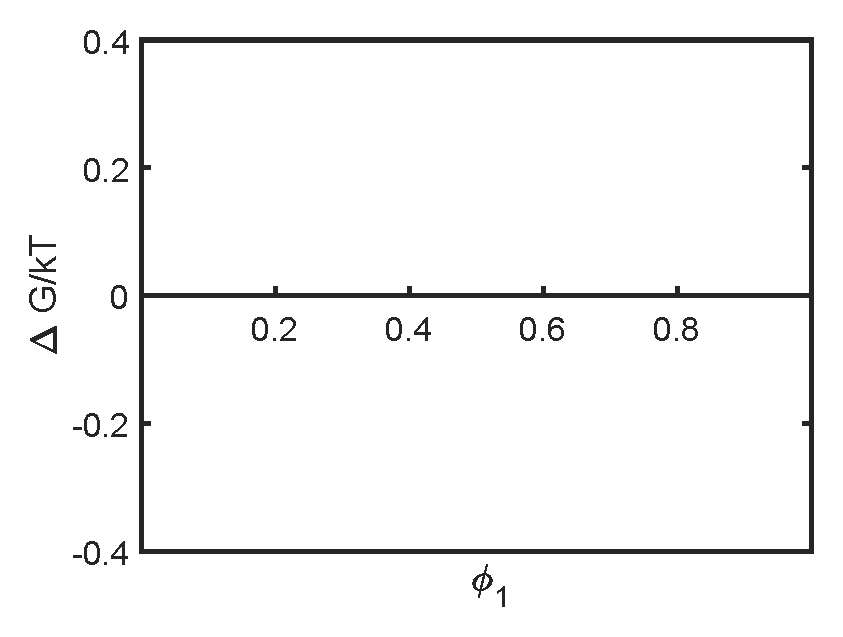
\includegraphics[width=\textwidth]{\figpath/model1-blankaxes}}
		\end{minipage}
		\begin{minipage}{0.3\textwidth}
			\centerline{$\chi = 0$, $N = 4$}
			
			\centerline{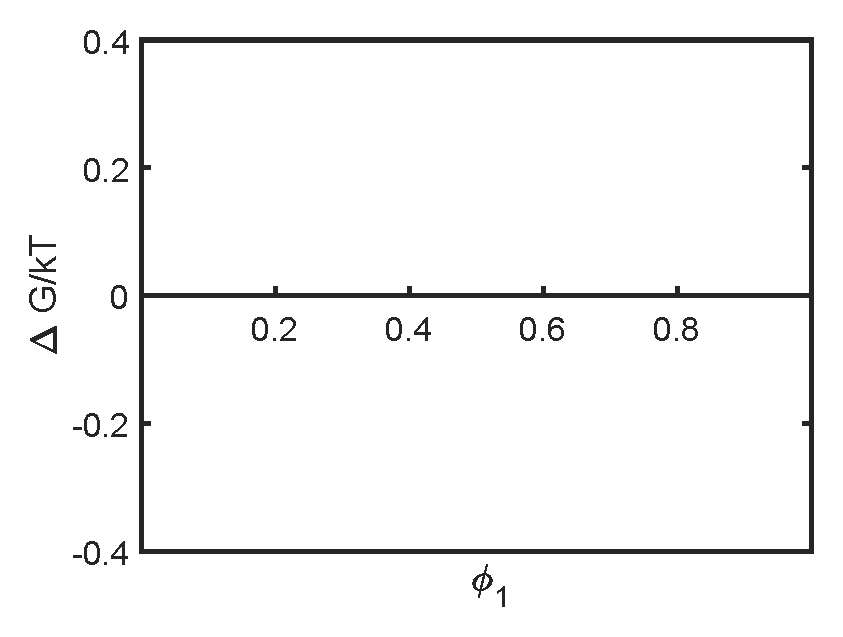
\includegraphics[width=\textwidth]{\figpath/model1-blankaxes}}
		\end{minipage}
	
		\vspace{0.1in}
		\begin{minipage}{0.3\textwidth}
			\centerline{$\chi = 2$, $N = 1$}
			
			\centerline{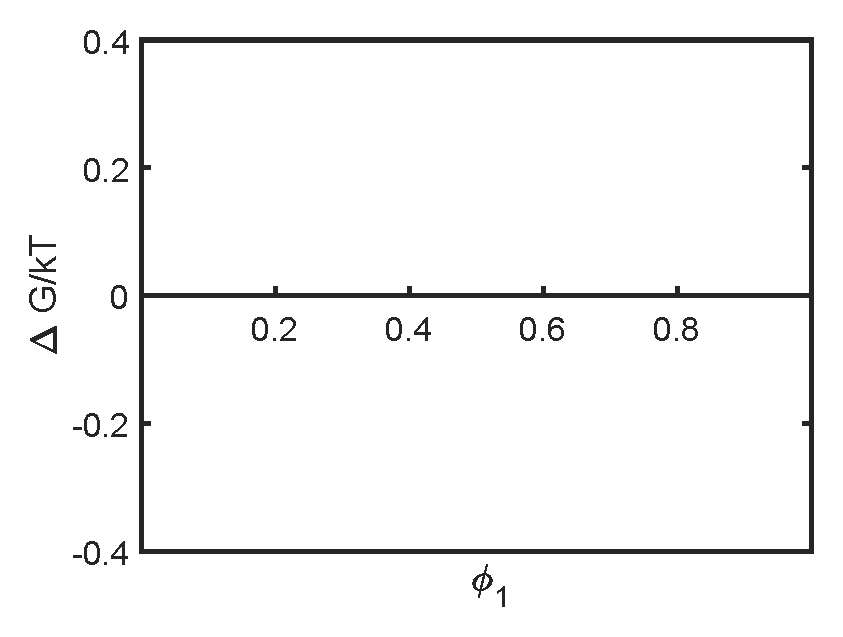
\includegraphics[width=\textwidth]{\figpath/model1-blankaxes}}
		\end{minipage}
		\begin{minipage}{0.3\textwidth}
			\centerline{$\chi = 2$, $N = 2$}
			
			\centerline{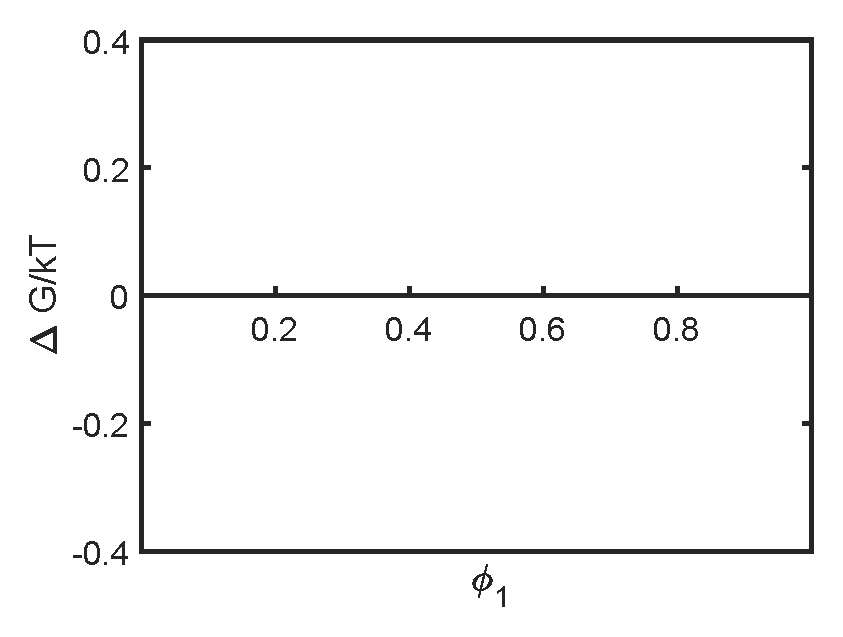
\includegraphics[width=\textwidth]{\figpath/model1-blankaxes}}
		\end{minipage}
		\begin{minipage}{0.3\textwidth}
			\centerline{$\chi = 2$, $N = 4$}
			
			\centerline{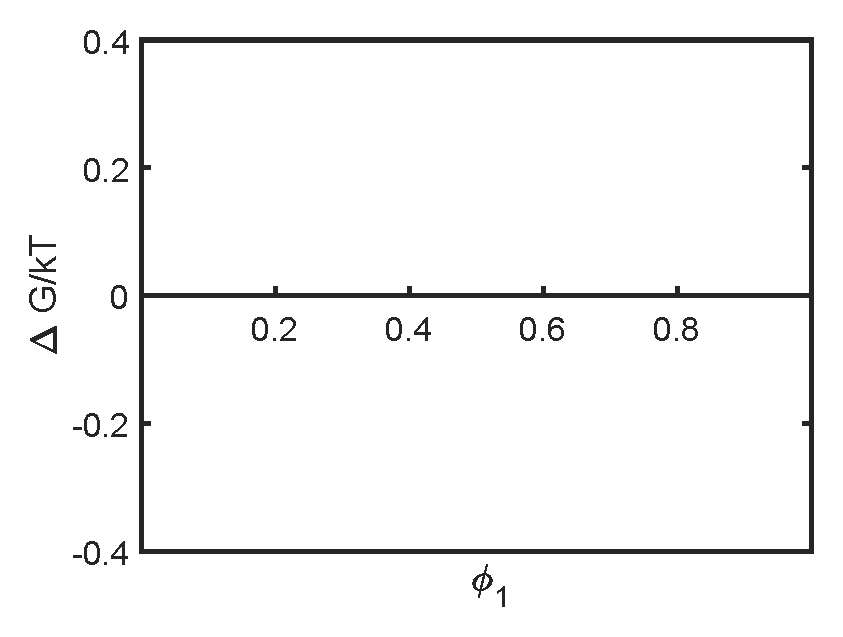
\includegraphics[width=\textwidth]{\figpath/model1-blankaxes}}
		\end{minipage}
	
		\vspace{0.1in}
		\begin{minipage}{0.3\textwidth}
			\centerline{$\chi = 4$, $N = 1$}
			
			\centerline{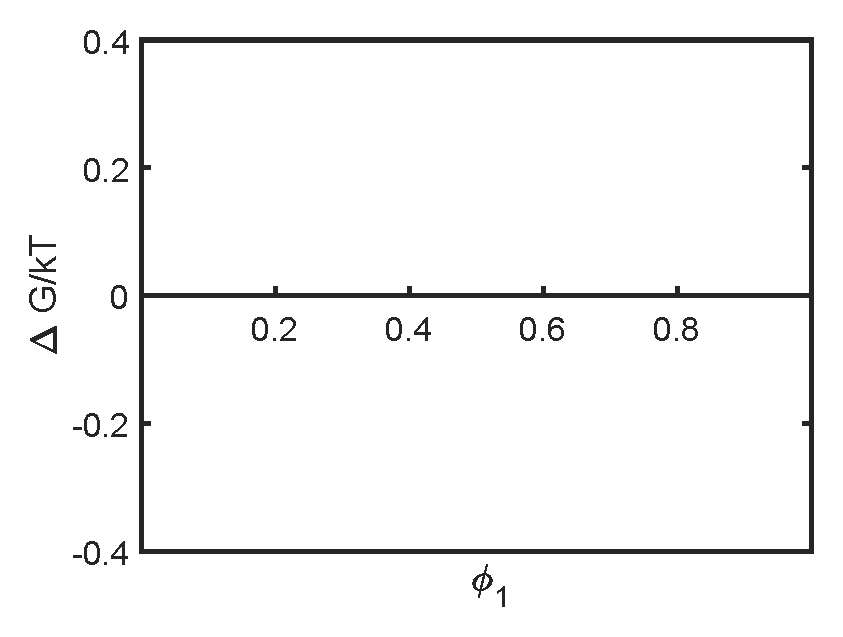
\includegraphics[width=\textwidth]{\figpath/model1-blankaxes}}
		\end{minipage}
		\begin{minipage}{0.3\textwidth}
			\centerline{$\chi = 4$, $N = 2$}
			
			\centerline{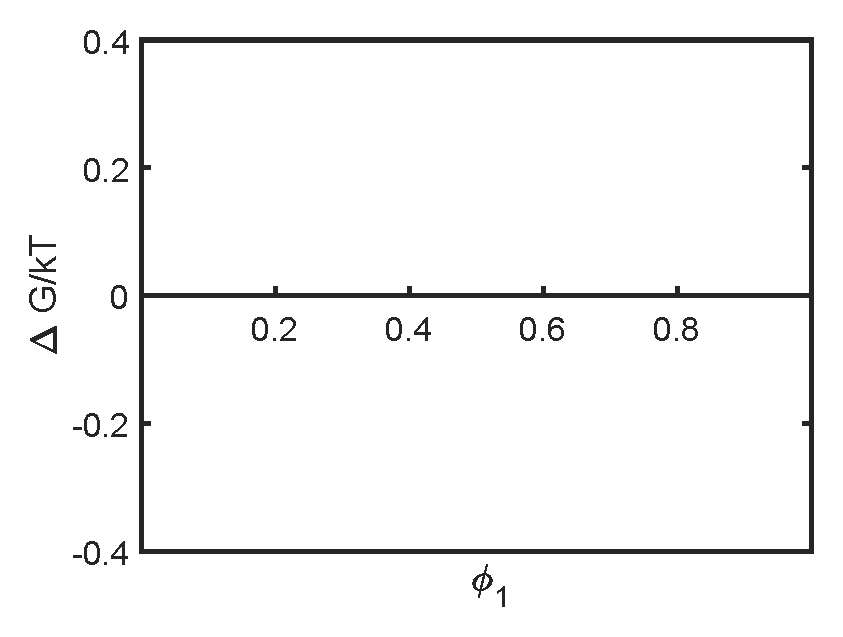
\includegraphics[width=\textwidth]{\figpath/model1-blankaxes}}
		\end{minipage}
		\begin{minipage}{0.3\textwidth}
			\centerline{$\chi = 4$, $N = 4$}
			
			\centerline{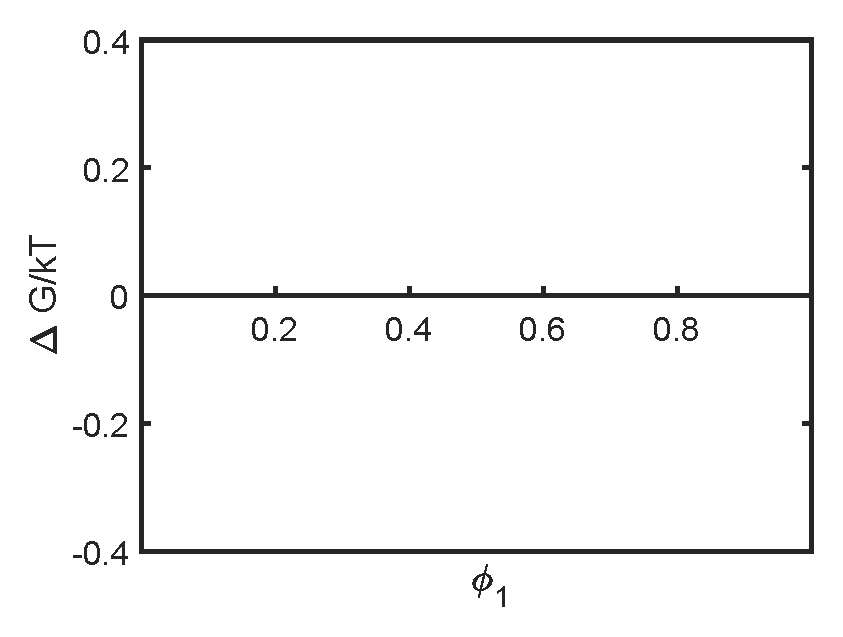
\includegraphics[width=\textwidth]{\figpath/model1-blankaxes}}
		\end{minipage}
	
	\question One of the plots you drew in the previous question corresponds to mixing two identical small-molecule liquids.  Which one is it?  Briefly justify your reasoning.
	
		\begin{solution}[2in]
		\end{solution}
	
	\question Describe, in 1-2 complete sentences, the changes in the free energy curve that result from...
		\begin{enumerate}
			\item ... increasing $\chi$:
	
				\begin{solution}[1.75in]
				\end{solution}
		
			\clearpage
			\item ... increasing $N$:
	
				\begin{solution}[1.75in]
				\end{solution}
		
		\end{enumerate}
		
\end{ctqs}



\begin{model}[Free Energy Changes on Phase Separation]

	When a polymer solution is prepared with a specific composition (that is, with a specific value of $\phi_1$), it can either remain a homogeneous, single-phase mixture with composition $\phi_1$, or it can phase separate into two new phases with different compositions, $\phi_{1A}$ and $\phi_{1B}$, as shown below:
	
		\centerline{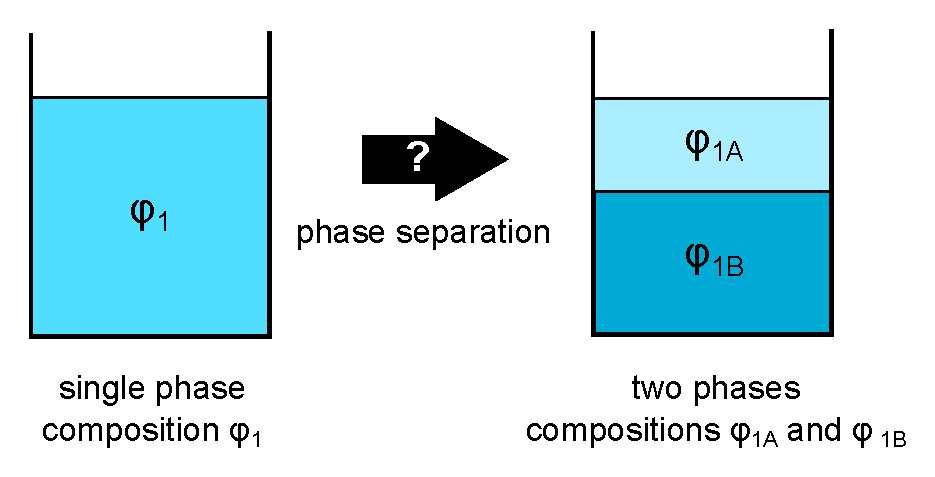
\includegraphics[width=0.65\textwidth]{\figpath/model2-schematic}}
	
	%When this phase separation occurs, the \emph{overall} composition of the sample does not change, but the compositions of the individual phases may be somewhat different from that of the starting mixture.
	
	Working through the math, it turns out that the free energy of the phase-separated mixture falls on a line connecting the free energies of the two individual phases:
	
		\vspace{0.1in}
		\centerline{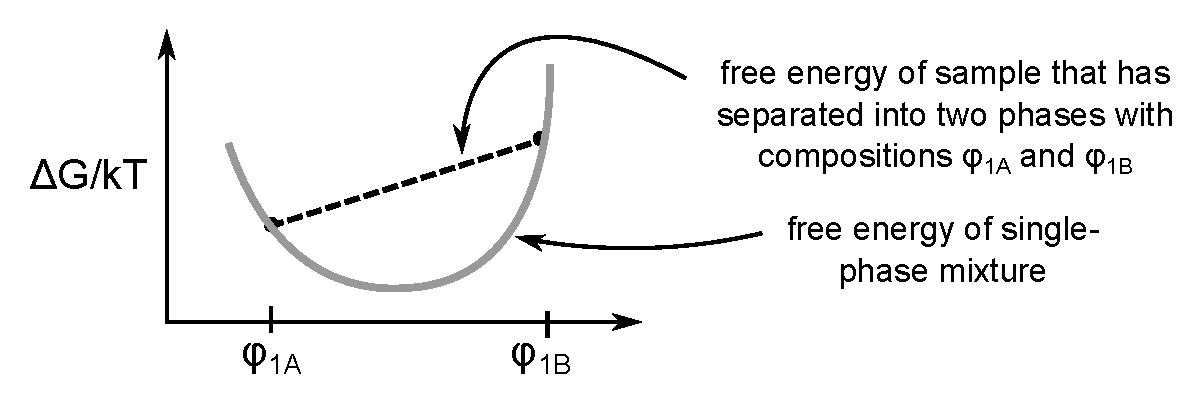
\includegraphics[width=0.8\textwidth]{\figpath/model2-deltaGphasesep}}
	
	If the free energy of the phase-separated mixture is lower than that of the homogeneous solution, the mixture will phase separate; otherwise, it will remain a single, stable phase.

\end{model}

		\vspace{0.1in}
\begin{ctqs}
		\question Consider a section of a free energy curve that is concave down, as shown below:
	
		\vspace{0.1in}
		\centerline{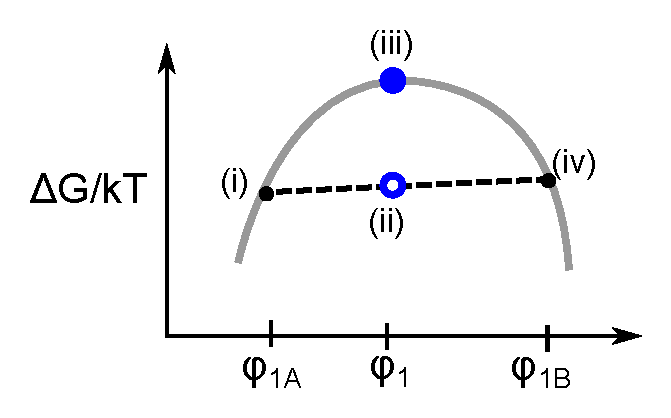
\includegraphics[width=0.5\textwidth]{\figpath/model2-concavedown}}

			\begin{enumerate}
				\item Which point on this plot represents a \emph{homogeneous solution} prepared at composition $\phi_1$?
					
					\begin{solution}[0.75in]
					\end{solution}
					
				\item Which point on this plot represents a mixture with total composition $\phi_1$ that has phase-separated into two phases with compositions $\phi_{1A}$ and $\phi_{1B}$, respectively?
					
					\begin{solution}[0.75in]
					\end{solution}
					
				\item Which state has the lower free energy, the phase-separated state or the homogeneous mixed state?
					
					\begin{solution}[0.75in]
					\end{solution}
					
				\item Will a sample prepared with overall composition $\phi_1$ spontaneously separate into two phases with compositions $\phi_{1A}$ and $\phi_{1B}$?  Why or why not?  Briefly explain your answer in 1-2 complete sentences.
					
					\begin{solution}[1.5in]
					\end{solution}
					
			\end{enumerate}
			
		\clearpage
		\question Next, consider a section of a free energy curve that is concave up, as shown below:
	
		\vspace{0.1in}
		\centerline{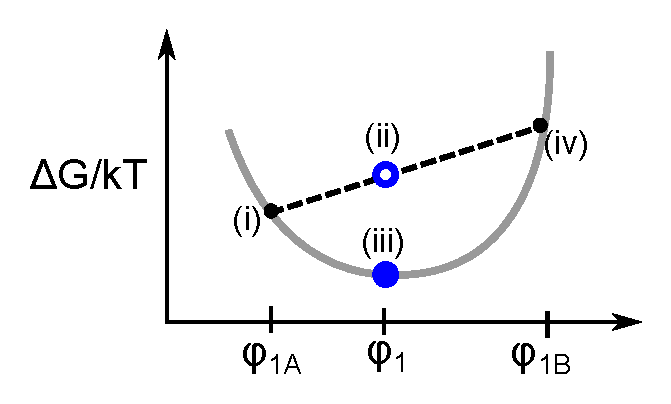
\includegraphics[width=0.5\textwidth]{\figpath/model2-concaveup}}

			\begin{enumerate}
				\item Which point on this plot represents a \emph{homogeneous solution} prepared at composition $\phi_1$?
					
					\begin{solution}[0.75in]
					\end{solution}
					
				\item Which point on this plot represents a mixture with total composition $\phi_1$ that has phase-separated into two phases with compositions $\phi_{1A}$ and $\phi_{1B}$, respectively?
					
					\begin{solution}[0.75in]
					\end{solution}
					
				\item Which state has the lower free energy, the phase-separated state or the homogeneous mixed state?
					
					\begin{solution}[0.75in]
					\end{solution}
					
				\item Will a sample prepared with overall composition $\phi_1$ spontaneously separate into two phases with compositions $\phi_{1A}$ and $\phi_{1B}$?  Why or why not?  Briefly explain your answer in 1-2 complete sentences.
					
					\begin{solution}[2in]
					\end{solution}
					
			\end{enumerate}
			
		\question We can describe these two cases mathematically by looking at the second derivative of $\Delta G$ with respect to $\phi_1$.		
			What is the \emph{sign} of $\frac{\partial^2 \Delta G}{\partial \phi_1^2}$ when...
			
			\begin{enumerate}
				\item ... the free energy curve is concave down?
					
					\begin{solution}[1in]
					\end{solution}
					
				\item ... the free energy curve is concave up?
					
					\begin{solution}[1in]
					\end{solution}
					
			\end{enumerate}
		
		\question Describe, in 2-3 complete sentences, how you could use the second derivative of $\Delta G$ to determine whether or not a mixture prepared at a given composition will phase separate.
					
					\begin{solution}[3in]
					\end{solution}
					
\end{ctqs}

\clearpage
\begin{model}[Phase Boundaries for Polymer Solutions]

The free energy curve for a polymer solution with $\chi > 0$ is shown below:

\centerline{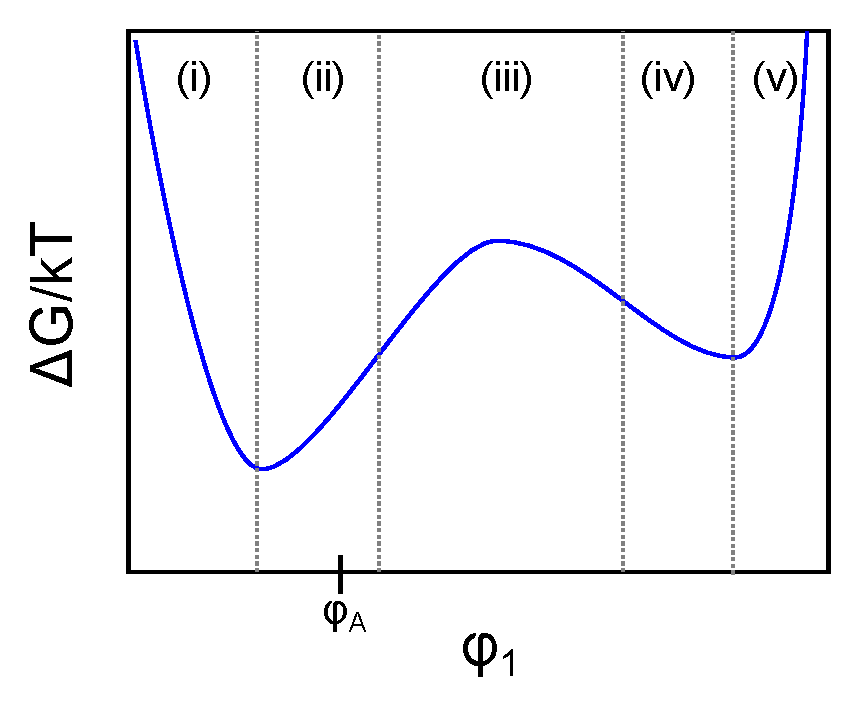
\includegraphics[width=0.5\textwidth]{\figpath/model3-regioncurve}}

\end{model}

\begin{ctqs}

		\question \label{ctq:regionconcavity} In what regions of this plot is the free energy curve...
			\begin{enumerate}
				\item ... concave up?
					
					\begin{solution}[0.75in]
					\end{solution}
				\item ... concave down?
					
					\begin{solution}[0.75in]
					\end{solution}
			\end{enumerate}
			
		\question \label{ctq:phaseseplocal} Based solely on your answers to question \ref{ctq:regionconcavity}, would you expect a mixture prepared with composition $\phi_1 = \phi_A$ to phase separate?  Briefly explain your reasoning.
					
					\begin{solution}[1.75in]
					\end{solution}
		
		\question \label{ctq:linebelow} Can you draw a line connecting \emph{any} two points on the free energy curve that would pass below the curve at $\phi_1=\phi_A$?
		
		\question \label{ctq:phasesepglobal} Based solely on your answer to question \ref{ctq:linebelow}, would you expect a mixture prepared with composition $\phi_1 = \phi_A$ to phase separate?
		
		\question Do your answers to questions \ref{ctq:phaseseplocal} and \ref{ctq:phasesepglobal} agree?  Why or why not?
			
\end{ctqs}

\begin{infobox}
	In polymer solutions, there are two different ways we can think about phase separation.
	
	First, if there is \emph{any} way to decrease the free energy by undergoing phase separation, then phase separation must be, overall, thermodynamically favorable.
	
	But separating into two phases with very different compositions requires big changes in the local composition, which can be slow, or kinetically unfavorable.
	
	So the second way to think about phase separation is to look just at the local concavity of the free energy curve.  If it is concave up, then any \emph{small} fluctuations in the local composition will increase the free energy and are unfavorable, so the mixture might not phase separate even if doing so could lower its overall free energy.  We refer to mixtures that are trapped this sort of local minimum as \emph{metastable}.
\end{infobox}

\begin{ctqs}
	\question In which regions of the plot shown in Model 3 do you expect mixtures to...
		\begin{enumerate}
			\item ... always phase separate?
			
			\item ... never phase separate?
			
			\item ... be metastable?
		\end{enumerate}
		
	\question In 2-3 complete sentences, briefly explain your reasoning for the previous question:
\end{ctqs}

\begin{infobox}
	The points that define the boundaries of the regions that will always spontaneously phase separate are called \emph{spinodal} points.
	
	The points that define the boundaries of the region where phase separation is thermodynamically favorable, even if it might not happen spontaneously, are called \emph{binodal} points.
\end{infobox}

\begin{ctqs}
	\question Locate and label the spinodal points (with an ``S'') and the binodal points (with a ``B'') on the free energy curve shown below:
	
	\question Propose a \emph{mathematical} method that you could use to find the spinodal points of an arbitrary free energy curve.  Describe your procedure in 2-3 complete sentences.
	
		\emph{Hint: remember that in the concave-up regions, $\frac{\partial^2\Delta G}{\partial \phi_1^2} > 0$ and in the concave-down regions, $\frac{\partial^2\Delta G}{\partial \phi_1^2} < 0$.  What must be true about this derivative at the points where the curve transitions between concave up and concave down?}
		
	\question Propose a \emph{graphical} method that you could use to find the binodal points on the free energy curve.  Describe your procedure using 2-3 complete sentences and any diagrams necessary to illustrate your approach.
\end{ctqs}



%\begin{exercises}

%		\exercise ...
%\end{exercises}
	
\end{activity}


\end{document}
